\documentclass[conference]{IEEEtran}
\IEEEoverridecommandlockouts
% The preceding line is only needed to identify funding in the first footnote. If that is unneeded, please comment it out.
%Template version as of 6/27/2024
\usepackage[utf8]{inputenc}
\usepackage{cite}
\usepackage{multirow}
\usepackage{enumitem}
\usepackage{textcomp}
\usepackage{makecell}
\renewcommand\theadfont{\bfseries} % Makes all \thead text bold by default
\usepackage{tcolorbox}

\newtcolorbox{databox}[1][]{
    colback=gray!10,      % Very light gray background
    colframe=black,       % Formal black border
    boxrule=0.5pt,        % Thin elegant line
    arc=0pt,              % Square corners (more formal than rounded)
    fonttitle=\bfseries\small,
    title=#1,
    fontupper=\small\ttfamily, % Typewriter font for content
    left=2pt, right=2pt, top=2pt, bottom=2pt
}

\usepackage{amsmath,amssymb,amsfonts}
\usepackage{algorithmic}
\usepackage{subfigure}
\usepackage{tabularx}
\usepackage{graphicx}
\usepackage{textcomp}
\usepackage{xcolor}
\usepackage{booktabs}
\usepackage{soul} % For \hl highlighting
\usepackage{svg}
\usepackage{url}
\usepackage{dblfloatfix}
\def\BibTeX{{\rm B\kern-.05em{\sc i\kern-.025em b}\kern-.08em
    T\kern-.1667em\lower.7ex\hbox{E}\kern-.125emX}}
\begin{document}

\title{
A TinyMoE Approach for Embedded Mixture-of-Experts in Driver Support Systems
\thanks{This work was financially supported by UID/00147 of SYSTEC and by the Associate Laboratory ARISE (LA/P/0112/2020), both funded by Fundação para a Ciência e a Tecnologia, I.P. (FCT) / MCTES through national funds, and by FCT through a PhD scholarship (2024.02446.BD).}
}


\author{
\IEEEauthorblockN{
Thommas K. S. Flores\IEEEauthorrefmark{1},
%
João Carlos N. Bittencourt\IEEEauthorrefmark{2}$^{,}$\IEEEauthorrefmark{3},
Thiago C. Jesus\IEEEauthorrefmark{2}$^{,}$\IEEEauthorrefmark{4},
%
Ivanovitch Silva\IEEEauthorrefmark{1},
Daniel G. Costa\IEEEauthorrefmark{2}
} 
\IEEEauthorblockA{\IEEEauthorrefmark{1}PPgEEC-UFRN, Federal University of Rio Grande do Norte, Natal, Brazil}%
\IEEEauthorblockA{\IEEEauthorrefmark{2}SYSTEC-ARISE, Faculty of Engineering, University of Porto, Porto, Portugal}%
\IEEEauthorblockA{\IEEEauthorrefmark{3}CETEC, Federal University of Recôncavo da Bahia, Cruz das Almas, Brazil}%
\IEEEauthorblockA{\IEEEauthorrefmark{4}DTEC-UEFS, State University of Feira de Santana, Feira de Santana, Brazil}%



Email: thommas.flores.101@ufrn.edu.br, joaocarlos@ufrb.edu.br, ivanovitch.silva@ufrn.br, \{danielgcosta, jesus\}@fe.up.pt}

\maketitle

\begin{abstract}
The deployment of natural language understanding capabilities on resource-constrained microcontrollers (MCU) is often limited by the trade-off between model capacity and memory footprint. This paper proposes TinyMoE, a system-level Mixture-of-Experts (MoE) architecture designed for automotive driver support systems. Unlike traditional MoE implementations that assume high-bandwidth memory swapping, the proposed approach utilizes an embedding-based semantic router to invoke independent, domain-specialized Small Language Models (SLMs) on-demand. We evaluate the proposed framework across seven MCU platforms, including ARM Cortex-M and Xtensa architectures. Experimental results show that TinyMoE significantly outperforms a monolithic global model, achieving lower training loss, faster inference on mid-range hardware, and higher exact match accuracy. These results validate system-level Mixture-of-Experts as an effective approach for multi-domain intelligence in bare-metal embedded environments, while preserving real-time performance under tight memory constraints. 
\end{abstract}

\begin{IEEEkeywords}
 TinyML, Small Language Models, Embedded Systems, Automotive Systems, Internet of Things.
\end{IEEEkeywords}



\section{Introduction}
\label{sec:introduction}

In automotive environments, drivers often require rapid access to information regarding traffic regulations, car operation, and emergency procedures. Retrieving accurate information within seconds is especially critical during mechanical failures, adverse weather conditions, or health emergencies. Although traditional vehicle manuals offer comprehensive reference material, they are typically dense and not structured for quick consultation \cite{electronics13244972,lee2023llmchatbot}. While cloud-based assistants provide interactive alternatives, their reliance on network connectivity introduces latency and availability challenges for in-vehicle applications \cite{surveyGenAI}. As a result, there is increasing interest in deploying natural language understanding capabilities directly on automotive embedded hardware. 

Recent advances in Tiny Machine Learning (TinyML) have established the feasibility of deploying compact neural networks on microcontroller units (MCUs) \cite{tinymlops}. Small Language Model (SLM) architectures and embedding compression techniques have further extended these capabilities to language tasks \cite{yang2023tinyformer, 10.1145/3676536.3676747}, making on-device natural language assistance increasingly viable. However, a single SLM must balance breadth and depth when encoding multiple domains within the limited parameter budget of an MCU. This tension between specialization and generalization reduces accuracy for heterogeneous queries, thereby motivating the development of lightweight mechanisms for domain specialization.


The Mixture-of-Experts (MoE) paradigm addresses this trade-off by routing heterogeneous queries to domain-specialized sub-networks, consequently expanding coverage without requiring a single monolithic model to manage all domains equally well. Recent research has adapted these concepts to edge platforms using hierarchical, memory-aware strategies such as expert preloading and adaptive quantization \cite{yi2025edgemoe}. However, they are designed for devices with memory budgets exceeding those of typical microcontrollers and generally assume that multiple experts are memory-resident during inference or can be swapped in rapidly. However, these assumptions do not hold for bare-metal MCU deployments.

To address these memory constraints, this paper introduces a system-level MoE architecture designed for resource-constrained MCUs. The proposed approach consists of training independent, domain-specialized SLM experts for traffic regulations, owner's manuals, and first aid, integrated with an embedding-based semantic router. During inference, the router assigns each query to a specific domain and loads only the corresponding expert, preserving specialization without requiring multiple experts to reside in RAM. This strategy shifts MoE from a within-model architectural choice to a between-model system design suitable for MCUs. Building on this formulation, the study makes three primary contributions: (i) reformulating MoE as a system-level design for memory-constrained MCUs to enable multi-domain natural language understanding via on-demand expert loading; (ii) designing an embedding-based semantic router and training domain-specialized SLM experts for automotive domains; and (iii) evaluating the approach on ESP32 and Arduino-based platforms under strict memory and latency constraints.

The remainder of this paper is organized as follows. Section~\ref{sec:related} reviews related works. Section~\ref{sec:approach} details the proposed approach, while Section~\ref{sec:case_study} outlines the considered case study. Section~\ref{sec:results} presents the experimental setup and results, followed by conclusions and references. 

\section{Related Work} 
\label{sec:related}

MoE models offer a strategy for deploying large neural networks under resource constraints. By using conditional computation to route tokens or queries to a subset of specialized experts, MoE models increase effective capacity without activating all parameters for each input. Early studies introduced sparsely-gated MoE layers and proved the feasibility of large-scale training with sparse routing \cite{shazeerOutrageouslyLargeNeural2017}. Subsequent work increased scalability through sharding and more efficient routing mechanisms \cite{lepikhinGShardScalingGiant2020,fedusSwitchTransformersScaling2021}. These architectures have demonstrated that sparse activation can deliver strong natural language processing performance while reducing inference costs, making them suitable for deployment in resource-limited edge environments. However, adapting MoE models to edge devices presents additional challenges, as memory and storage bandwidth often become critical bottlenecks. The EdgeMoE framework handles these issues by separating always-on weights from expert weights stored externally and preloading experts as needed to minimize input/output latency \cite{yi2025edgemoe}. Nevertheless, this approach still assumes resource-rich scenarios based on smartphones or single-board computers. 

To address these challenges, TinyML research has advanced transformer-based language processing on edge devices by using architectural co-design, pruning, and specialized inference engines \cite{yang2023tinyformer}. Studies such as MobileLLM examine architectural methods that improve performance within limited parameter budgets on mobile-class hardware \cite{liu_mobilellm_2024}. For MCUs, TinyFormer and associated toolchains show that aggressive compression and hardware-aware optimization enable language inference under stringent SRAM constraints \cite{yang2023tinyformer}. MCUBERT addresses the embedding-table bottleneck through structured approximation, supporting longer input sequences within MCU SRAM limitations \cite{10.1145/3676536.3676747}. Additionally, deployment frameworks and compiler support improve efficiency on emerging heterogeneous MCU platforms \cite{scherer2024deeploy}. However, most existing systems focus on optimizing a single model and do not consider multi-domain assistants. 

Previous studies on manual question answering frequently reformulate the task as classification over a fixed set of intents or Frequently Asked Question (FAQ) categories, prioritizing predictable latency and memory usage over generative flexibility \cite{electronics13244972}. While cloud-based assistants and document Question Answering (QA) tools deliver adaptable interfaces, they introduce dependencies on connectivity and availability, which are unsuitable for in-vehicle environments \cite{lee2023llmchatbot}. Consequently, there is a need for on-device mechanisms capable of identifying the domain of a query and invoking only the necessary resources to generate a response. This paper fills this gap by presenting a system-level MoE design that routes queries to independent, automotive-specialized SLM experts, loading only the required expert into constrained MCU memory.

% ################
\section{Proposed Approach} \label{sec:approach}

\subsection{Data Acquisition}

The data used in this work were collected from three distinct sources, all provided as official PDF documents: (i) a first-aid manual, (ii) the applicable traffic regulations, and (iii) a vehicle owner’s manual. These documents constituted the study’s knowledge base and were segmented into passages of up to 100 characters. This empirical limit was defined through a supervised analysis, aiming to balance context preservation with the model’s limited context window.



\subsection{Knowledge Extraction}
\label{sec:knowledge_extraction}

A dataset was synthesized through a methodical pipeline designed to transform the raw content extracted from the PDF sources into a structured, instruction-following format. Textual content was extracted from the three documents (first aid manual, traffic regulations, and vehicle owner’s manual), leveraging PDF parsing to handle complex layouts and graphical elements. Then, the text was segmented into semantically coherent chunks. Rather than applying a simple fixed-length split, the algorithm respected natural paragraph boundaries in the source material. Consecutive paragraphs were grouped until a predefined token threshold was reached, at which point a new chunk began. This ensures each chunk retains a self-contained idea or procedural description, balancing contextual integrity with computational practicality for model training.

Finally, each chunk was converted into a question and answer pair using a Retrieval Augmented Generation (RAG) system built on the LLaMA~3.2 model \cite{dubey2024llama}. The system operated in a strictly local and offline environment to prevent external knowledge leakage and web based hallucinations. For each document, 500 question and answer pairs were generated, totaling 1500 pairs across the three sources. The dataset was split on a per-document basis, with 80\% used for training and 20\% used for testing. The RAG system was used only during this offline dataset generation phase; the final assistant model operates entirely offline, without any retrieval component.

The resulting instruction response pairs were stored in JSONL format, facilitating fine-tuning and reproducibility. Table~\ref{tab:qa_examples} presents representative examples of the generated pairs.



\begin{table}[htpb] % Note: table, not table*
\small
\centering
\caption{Representative question and answer pairs.}
\label{tab:qa_examples}

\newcolumntype{L}{>{\raggedright\arraybackslash}X}
\begin{tabularx}{\linewidth}{@{} 
    >{\hsize=1.4\hsize}L 
    >{\hsize=0.9\hsize}L 
    >{\hsize=0.7\hsize}L @{}}
\toprule
\textbf{Question} & \textbf{Answer} & \textbf{Source} \\
\midrule
What is autopilot mode for right scroll wheel?
& Autopilot mode.
& \textit{Owner's Manual} \\
\addlinespace

What should be done after an emergency?
& Clean up the affected area.
& \textit{First Aid} \\
\addlinespace

What is required to drive legally?
& A valid driving licence.
& \textit{Traffic Reg.} \\
\bottomrule
\end{tabularx}
\end{table}

\subsection{Preprocessing, Curation, and Tokenization}

Before training, we applied a structured preprocessing and curation pipeline to improve dataset quality, consistency, and domain relevance. We removed duplicate entries, incomplete samples, and ill formed question and answer pairs, as well as cases where the question was not supported by the corresponding answer. We also filtered out noisy examples, layout extraction artifacts, and content outside the target domain to mitigate bias and improve training stability.

The remaining samples were normalized through a lightweight cleaning procedure that removed redundant symbols, standardized punctuation, and harmonized casing and formatting. The cleaned sequences were then tokenized into integer identifiers required by the training framework. Special tokens represent padding (\texttt{<pad>}), sequence start (\texttt{<sos>}), sequence end (\texttt{<eos>}), unknown tokens (\texttt{<unk>}), and the delimiter between the question and the answer (\texttt{<sep>}).


\subsection{Expert Model Architecture}

The proposed model adopts a decoder-only Transformer architecture with masked multi-head causal self-attention. Unlike encoder based models such as BERT, which use bidirectional attention, causal masking restricts each position $t$ to attend only to positions $\le t$, preserving the autoregressive property required for next-token generation.

As shown in Fig.~\ref{fig:expert_architecture}, the model comprises token embeddings, positional encodings, a stack of Transformer blocks, and a final linear projection layer. Each Transformer block includes Layer Normalization, masked multi-head causal attention, residual connections, and a feed-forward network with Gaussian Error Linear Unit (GeLU) activation. This design supports deployment on MCU class devices by allowing the architecture depth and the number of attention heads to be tuned to available compute and memory.

\begin{figure}[htpb]
\centering
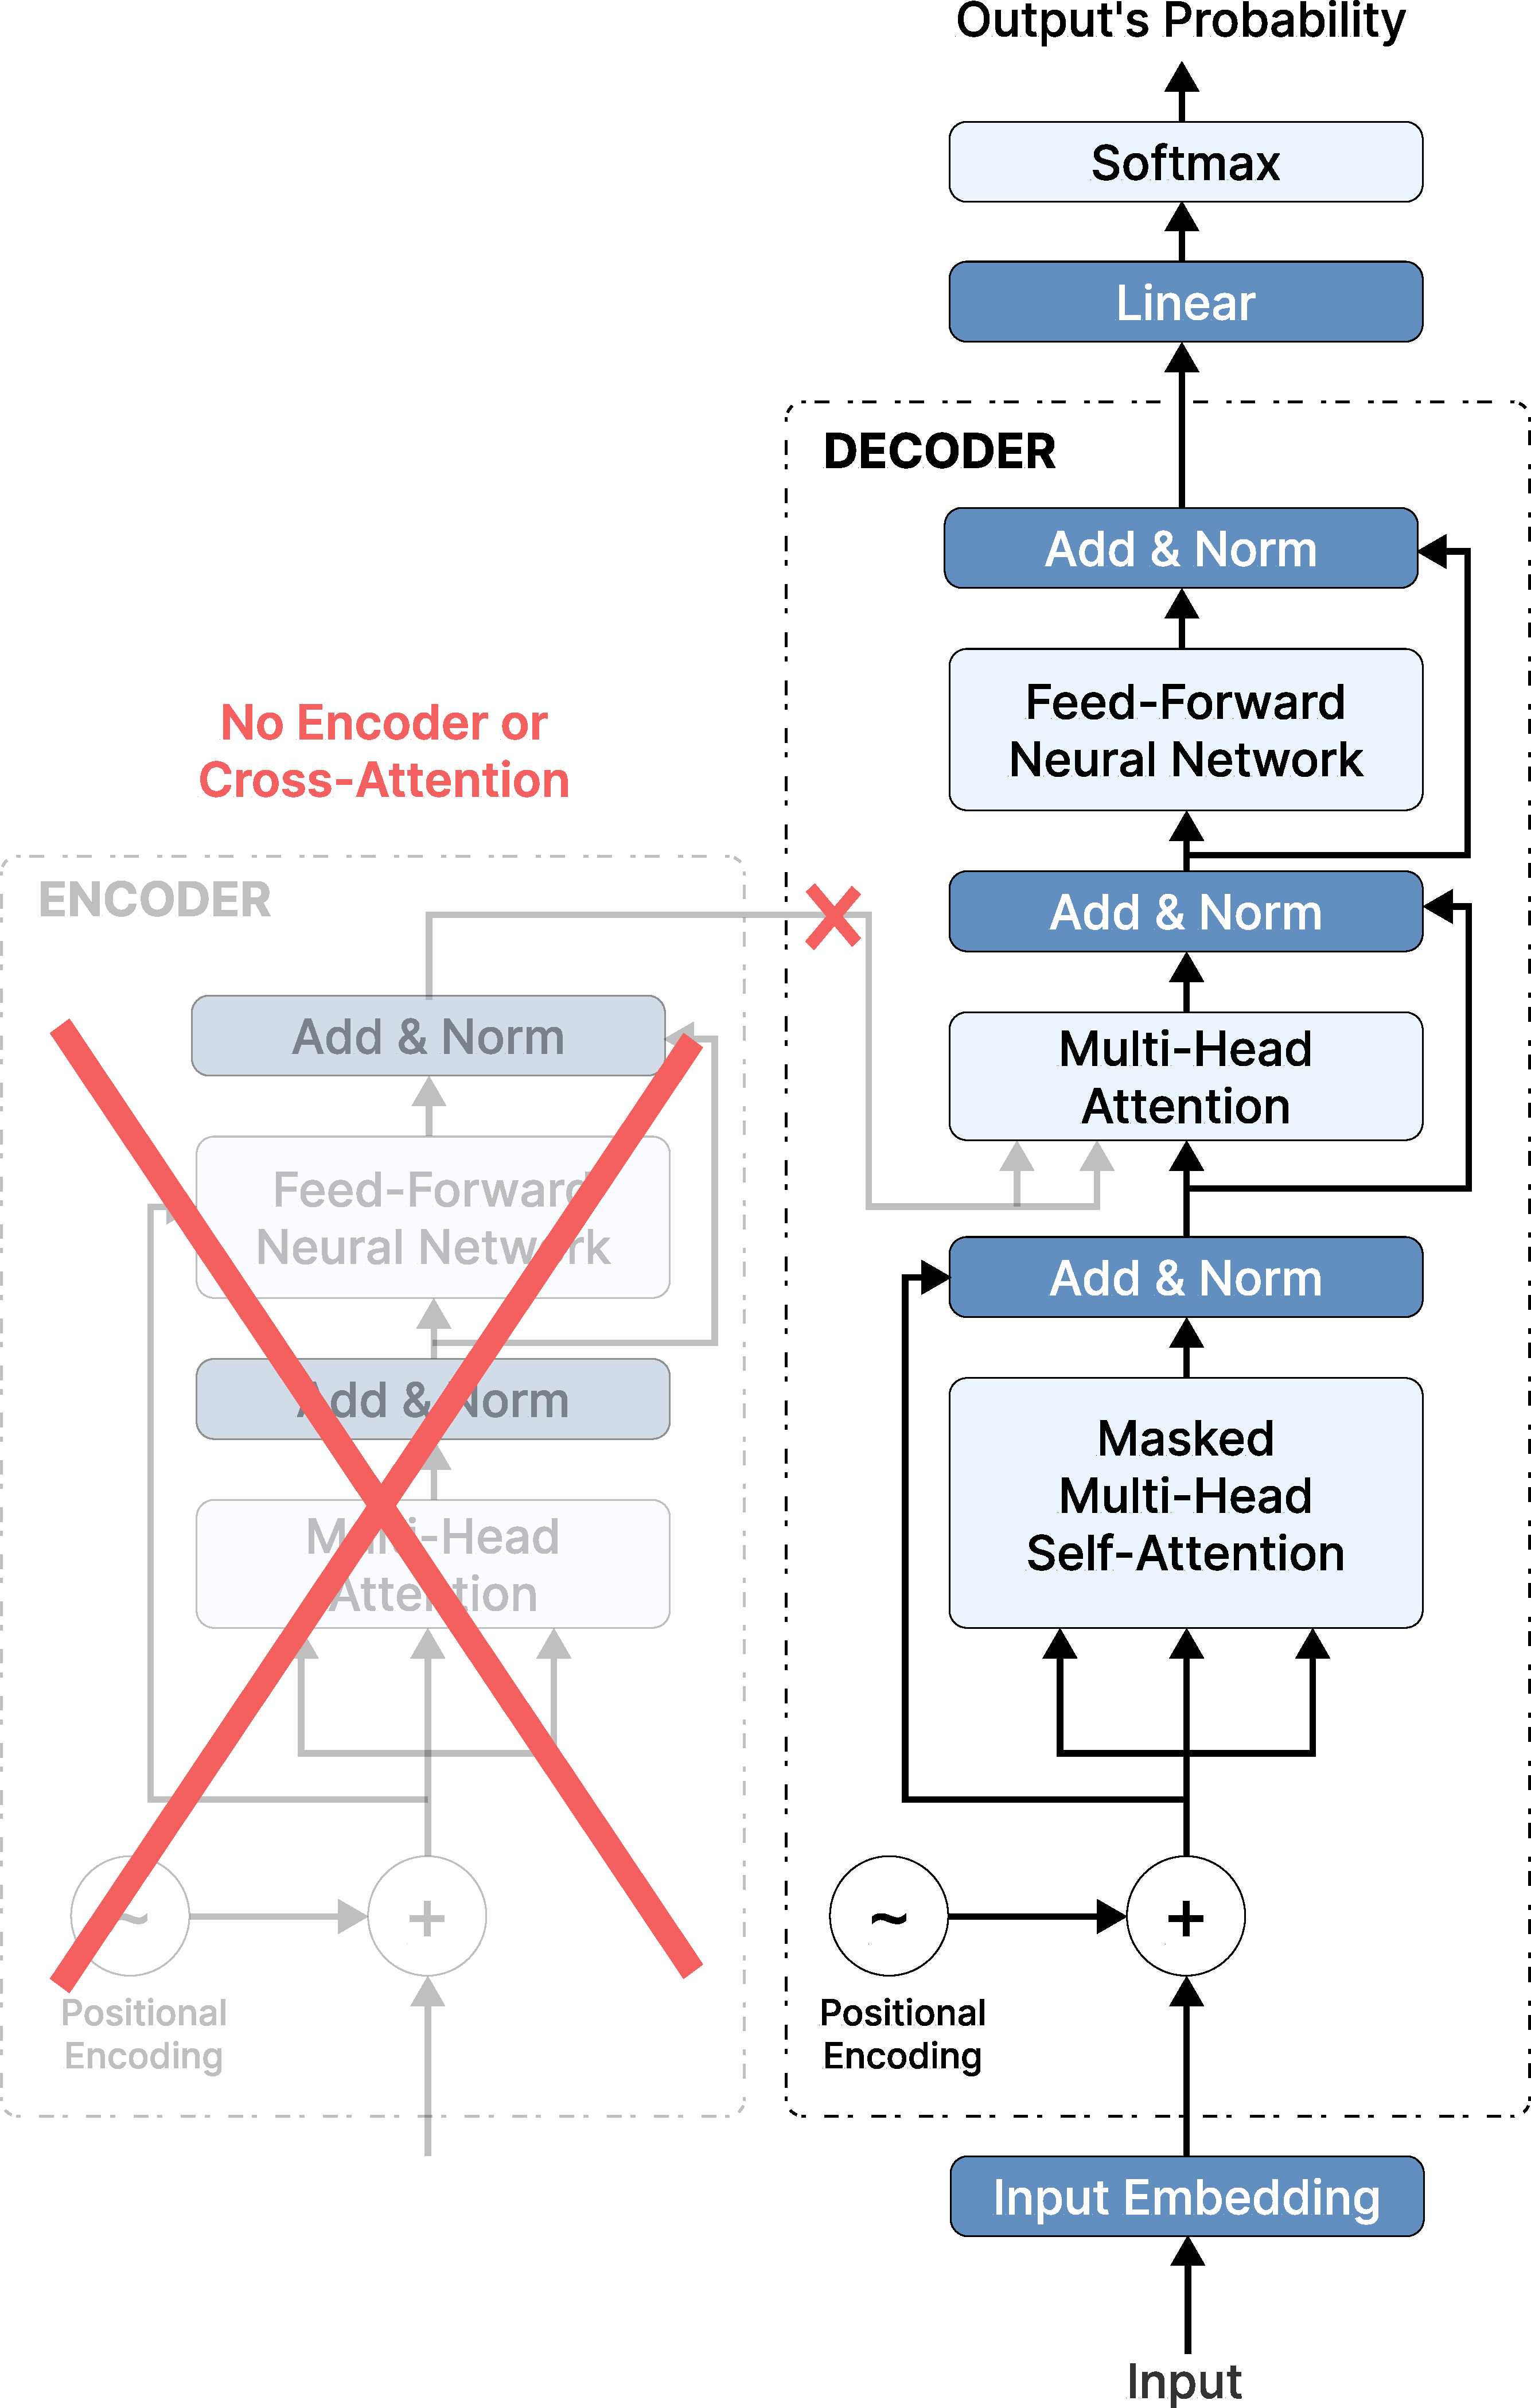
\includegraphics[width=0.75\linewidth]{Figures/expert_architecture.pdf}
\caption{TinyMoE expert architecture based on a decoder-only Transformer with masked causal self-attention.}
\label{fig:expert_architecture}
\end{figure}

During inference, the model generates text iteratively within a 32 token context window. At each step, it predicts the next token, appends it to the input sequence, and repeats the forward pass. This procedure follows the standard GPT style decoding process and does not require a separate encoder or retrieval component.



\subsection{Routing Mechanism}
\label{sec:router}

A MoE system uses a routing mechanism, also called a gating network, to select which expert processes each input query \cite{shazeerOutrageouslyLargeNeural2017}. In TinyMoE, routing is implemented with a Multinomial Naive Bayes (MNB) classifier.

As illustrated in Fig.~\ref{fig:gate_mechanism}, the input query $x$ is converted into a Bag-of-Words (BoW) representation. Given a vocabulary $V$, the query is encoded as a feature vector $f = [w_1, w_2, \dots, w_{|V|}]$, where $w_i$ is the frequency of the $i$th term in $x$. The router selects an expert $E_k \in \{E_{\text{first\_aid}}, E_{\text{owner\_manual}}, E_{\text{regulation}}\}$ by computing the posterior probability $P(E_k \mid f)$ using Bayes' theorem:

\begin{equation}
P(E_k \mid f) \propto P(E_k) \prod_{i=1}^{|V|} P(w_i \mid E_k)^{f_i}.
\end{equation}

Here, $P(E_k)$ is the prior probability of expert $E_k$, and $P(w_i \mid E_k)$ is the conditional probability of observing token $w_i$ under that expert. Parameters are estimated offline using Laplace smoothing to handle out-of-vocabulary (OOV) tokens.

\begin{figure}[htpb]
\centering
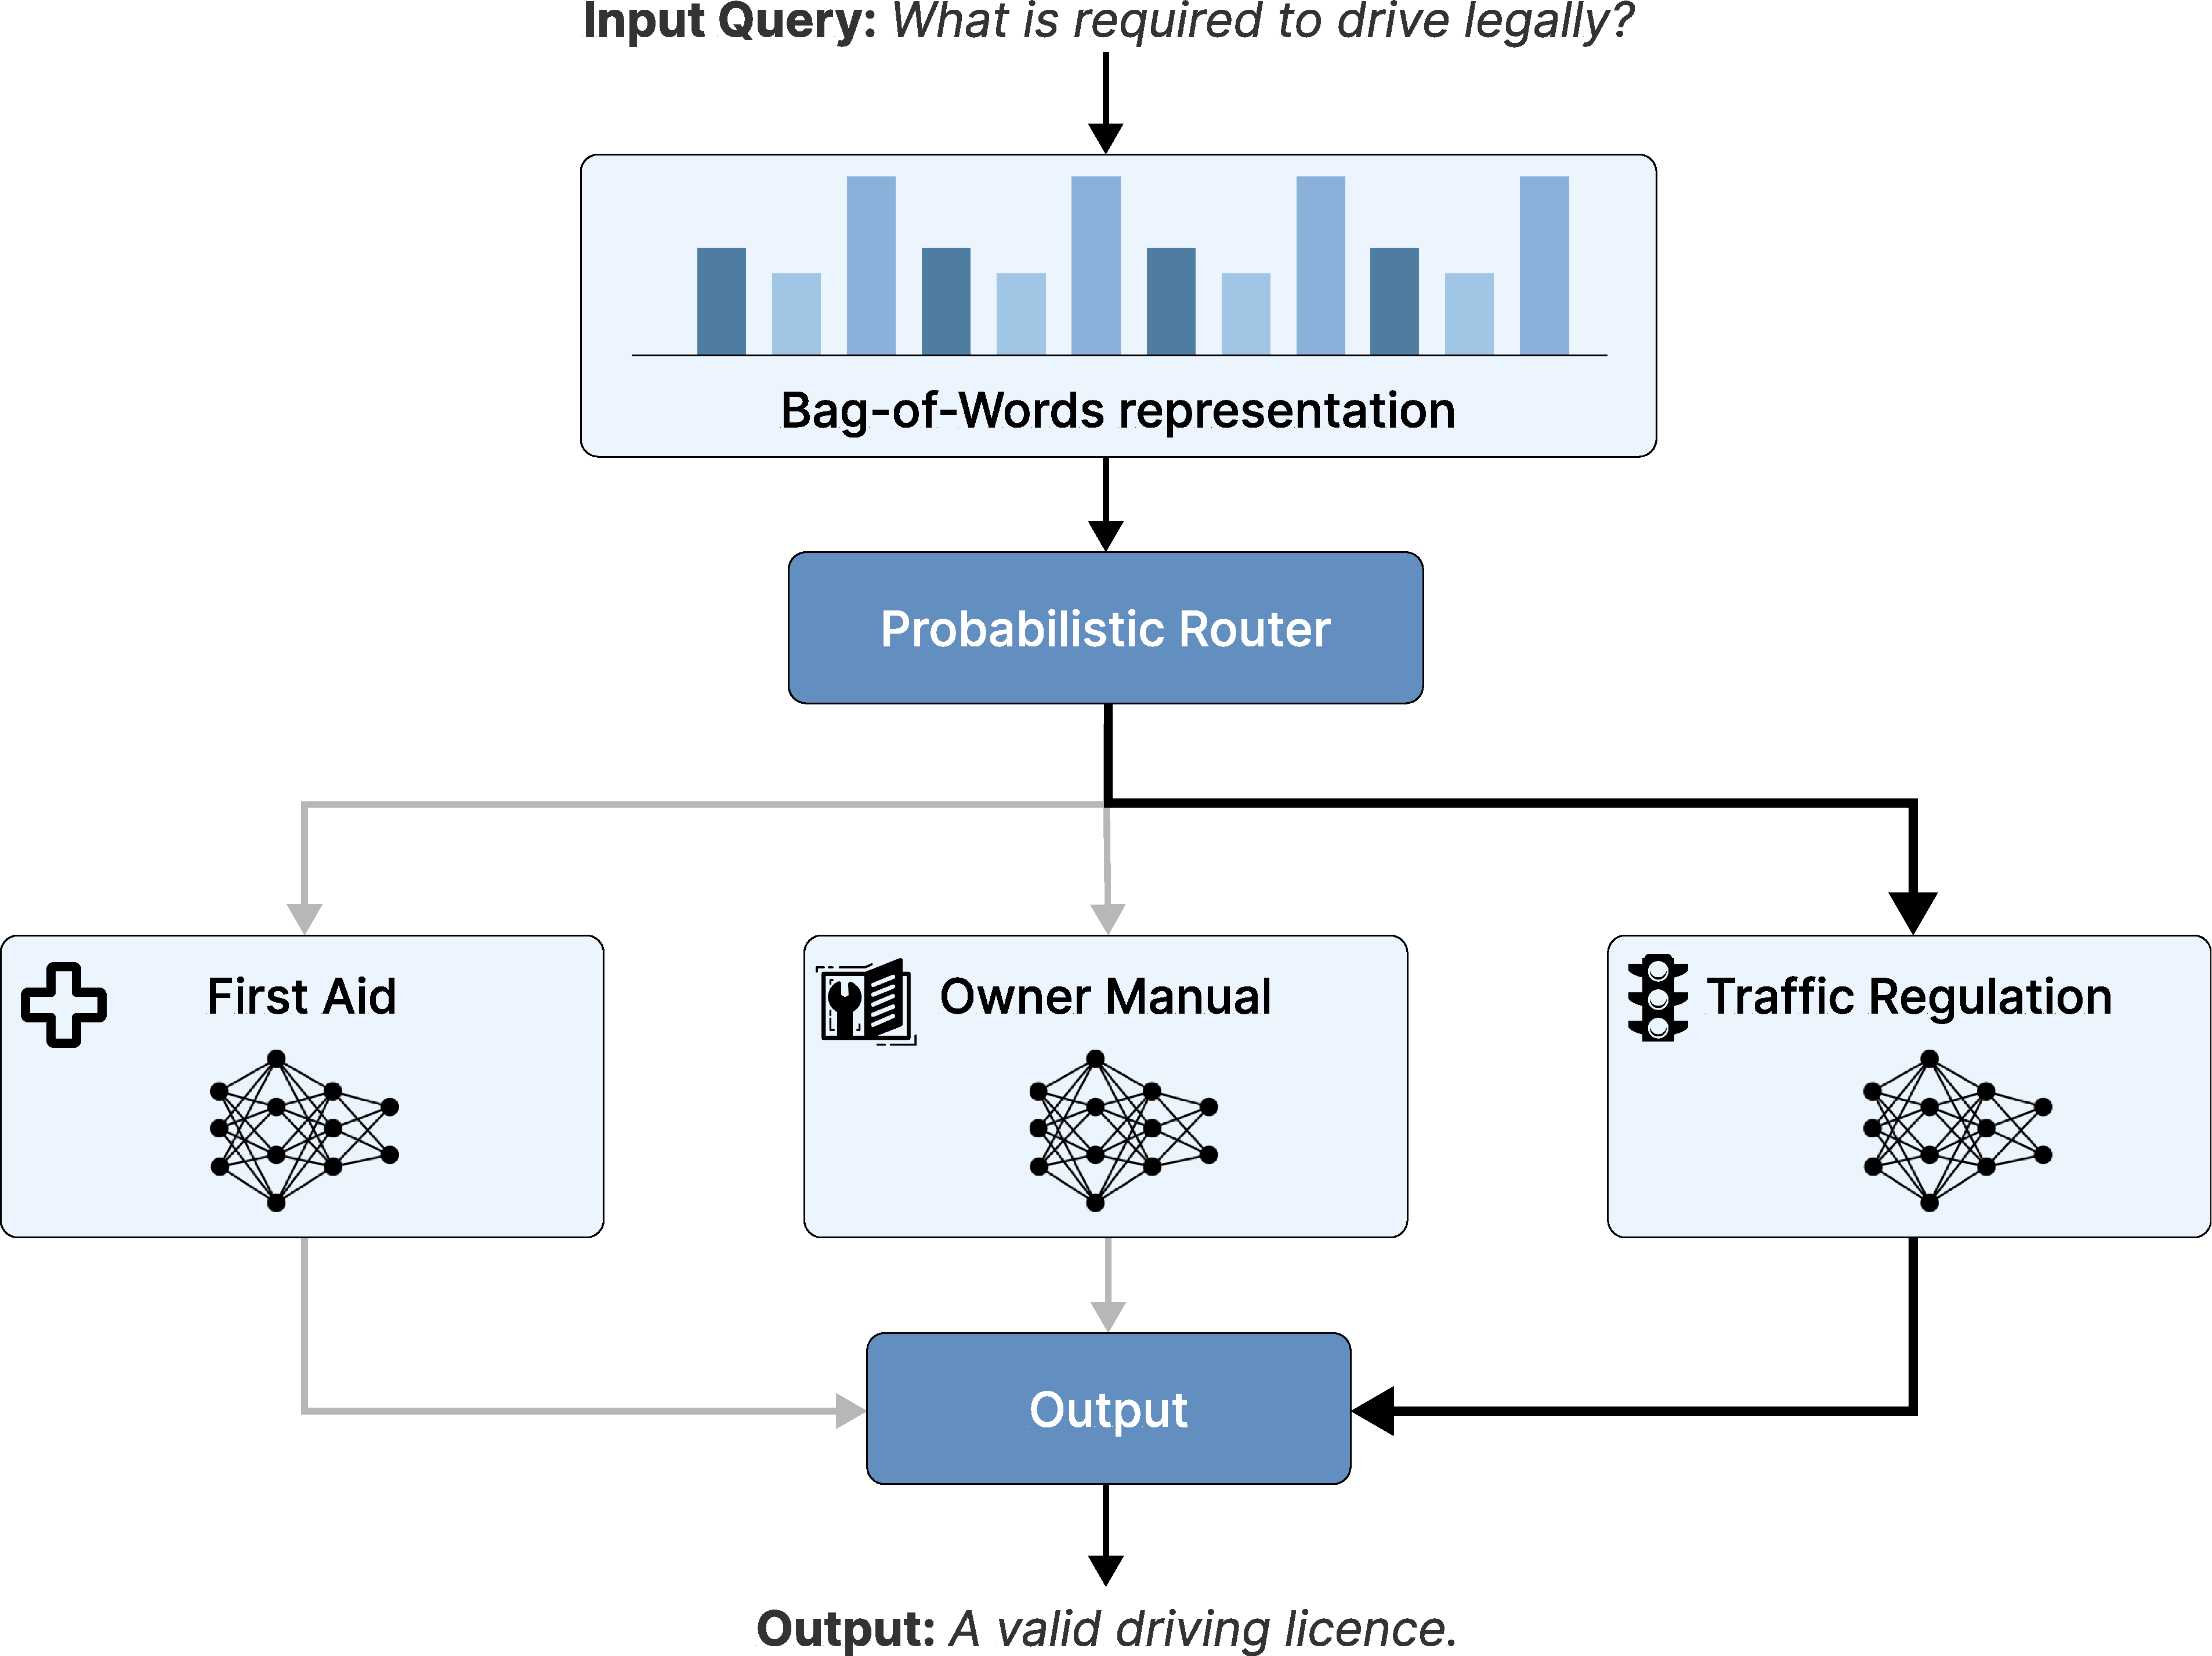
\includegraphics[width=0.95\linewidth]{Figures/gate_mechanism.pdf}
\caption{TinyMoE routing mechanism. The input query is converted into a Bag-of-Words representation. The router selects one expert by maximizing the log posterior probability. The final output is generated only by the selected expert.}
\label{fig:gate_mechanism}
\end{figure}

Compared with neural gating and Top-K routing \cite{fedusSwitchTransformersScaling2021}, inference is performed in the log-probability domain, converting products into sums:

\begin{equation}
\text{Route}(x) = \arg\max_{k} \left[ \log P(E_k) + \sum_{i \in x} \log P(w_i \mid E_k) \right].
\end{equation}

This design supports deployment on microcontroller-class devices by limiting computation and parameter storage. Each expert receives queries routed to its target domain, which reduces cross-domain interference \cite{puigcerver2024sparse}.




\subsection{Expert and Routing Mechanism Training}
The training process consists of two distinct stages: the supervised learning of a routing classifier and the independent optimization of domain-specific generative experts. The routing mechanism utilizes a Multinomial Naive Bayes (MNB) algorithm~\cite{10.1007/978-981-10-5041-1_57}. This classifier was trained on a dataset of 1,496 samples categorized into three domains: first aid, vehicle owner's manuals, and traffic regulations. Textual features were processed via a Bag-of-Words (BoW) representation, resulting in a router vocabulary of 1,579 tokens. The model parameters were fitted to minimize the negative log-likelihood of the domain labels given the feature distributions.

The expert models are based on a TinyGPT architecture, trained on synthetic question-answer pairs for domain-specific sequence modeling. The vocabulary for this stage comprises 1,707 unique tokens, with a maximum context length fixed at 23 tokens to minimize memory consumption on MCU. The model configuration includes a 12-dimensional embedding space, two attention heads, and a single transformer layer. A dropout rate of 0.01 was applied during training to prevent overfitting in the specialized corpus.

Optimization was conducted using the AdamW algorithm with a fixed learning rate of $1 \times 10^{-2}$ and a categorical cross-entropy loss function. The training was executed for 100 epochs with a batch size of 4. This training configuration ensures that each expert remains isolated within its respective semantic domain. The synergy between the MNB-based routing and the specialized expert training reduces cross-domain interference and enables efficient execution in resource-constrained embedded environments.


\subsection{Expert and Router Export for Embedded Deployment}
\label{sec:export_codegen}

After training, we export both parts of TinyMoE: the domain experts and the routing model. The goal is to translate the trained components into an embedded representation that can run on MCU. Each expert is serialized into an intermediate format that stores the architecture configuration, vocabulary, and learned parameters. The exported state includes embedding weights, Transformer block parameters, normalization coefficients, and the output projection, together with metadata such as depth, attention structure, and embedding dimensionality. This representation allows each expert to be reconstructed as an independent module.

In parallel, we export the Multinomial Naive Bayes router by serializing class priors, class conditional token log-probabilities, the routing vocabulary, and expert identifiers. This preserves the routing behavior learned during training.

Next, a code generation toolchain converts the exported artifacts into C++ source files for the experts and the router. For the experts, the generated code implements autoregressive inference, including token embedding, masked causal self-attention, feed-forward layers, normalization, and output logits. For the router, the generated module accumulates token log-likelihoods and selects the expert with a maximum a posteriori rule.

Model parameters are emitted as static arrays, and constants and function interfaces are exposed through header files. Parameter arrays can be placed in non-volatile memory to reduce RAM usage. The result is a self-contained implementation of TinyMoE for embedded inference under compute and memory constraints.


\subsection{Embedded Inference}
\label{subsec:embedded_inference}

At runtime, TinyMoE follows an inference pipeline. User queries are received through a serial interface and undergo minimal preprocessing, such as trimming whitespace and normalizing case, to match the routing vocabulary. The preprocessed query is passed to the router, which maps the query to a single domain and activates the corresponding expert (first aid, vehicle owner’s manual, or traffic regulation). This decision is made once per query. Next, the selected expert generates the answer autoregressively using the decoder-only Transformer described earlier. Inference uses a fixed-size output buffer and a predefined limit on the number of generated tokens to bound memory usage and runtime. Finally, the answer is returned to the user through the serial interface, optionally with on-device timing measurements. The system does not combine outputs from multiple experts; the response is produced only by the selected expert.

\section{Case Study}
\label{sec:case_study}

The proposed TinyMoE framework was evaluated through a structured case study focused on resource-constrained deployment, according to the following research questions:


\noindent \textbf{RQ1:} To what extent does the distributed parameter architecture of TinyMoE mitigate the capacity saturation and gradient interference observed in monolithic Global Models for multi-domain automotive tasks? 

\noindent \textbf{RQ2:} How does the semantic routing mechanism affect inference latency across heterogeneous MCU architectures compared to a generalist baseline with similar parameter counts? 

\noindent \textbf{RQ3:} What is the quantitative impact of expert specialization on the ratio between non-volatile storage overhead and real-time responsiveness in resource-constrained environments? 

The experimental setup involved training and preprocessing on a workstation equipped with an Intel® Core™ i5-8265U CPU (1.60--1.80~GHz) and 32~GB of RAM. To validate performance across a spectrum of embedded architectures, experiments were conducted on a diverse set of MCUs covering a wide range of computational and memory constraints. The Arduino Portenta H7 represents the high-performance end of the spectrum. Mid-range platforms include the ESP-WROOM-32 DEVKit V1 and the Raspberry Pi Pico~2 and Pico~2~W. Lower-end devices comprise the Raspberry Pi Pico and Pico~W and the Arduino Nano~33 BLE Sense. Collectively, these platforms reflect the heterogeneity of modern IoT edge nodes and enable a systematic evaluation of model behavior under varying computational and memory budgets.

The complete implementation is hosted in a public repository~\cite{tinyMoE}.

\subsection{Evaluation Metrics}
\label{subsec:eval_metrics}



The proposed approach is evaluated using a two-stage framework that covers both language generation quality and the constraints imposed by embedded deployment. During training and validation, the optimization objective and generation quality are assessed using the several metrics. \textbf{Cross-Entropy Loss} is the optimization objective and \textbf{Perplexity} measures uncertainty in next-token prediction, with lower values indicating better fit to the training distribution. \textbf{Token Accuracy} measures the fraction of correctly predicted tokens, while \textbf{Exact Match} requires the full generated sequence to match the reference. \textbf{BLEU} is reported to compare generated answers with reference responses.

Once deployed on the MCU, the evaluation shifts to physical constraints and real-time performance. \textbf{Inference Latency} represents the wall-clock time required to process an input and produce a complete response, measured directly on the device. Regarding the \textbf{Memory Footprint} (Flash vs. RAM), non-volatile Flash usage (for weights and code) is reported separately from peak RAM usage (for runtime buffers and activations) to verify compatibility with the MCU constraints.




\section{Results} \label{sec:results}
This section presents the results of evaluating the scenarios defined in Section~\ref{sec:case_study}.

\subsection{Routing Mechanism Evaluation}
\label{subsec:routing_evaluation}

We evaluated the router as a multi-class classifier to measure how often it assigns queries to the correct domain. We report results on the training and test splits using standard classification metrics and the confusion matrix in Fig.~\ref{fig:confusion_matrix}.



\begin{figure}[!htpb]
            \centering
            
            \subfigure[Test.]{
             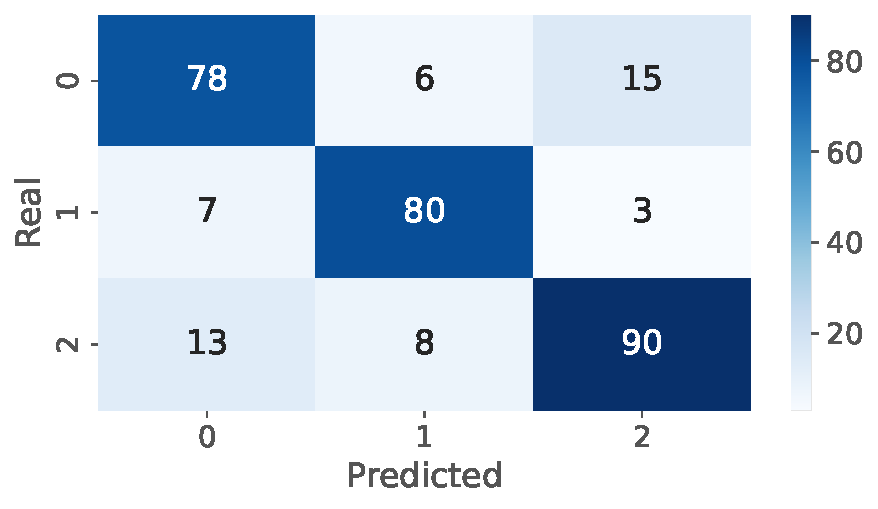
\includegraphics[width=.46\linewidth]{Figures/confusion_matrix_test}
            }
            \subfigure[Train.]{
              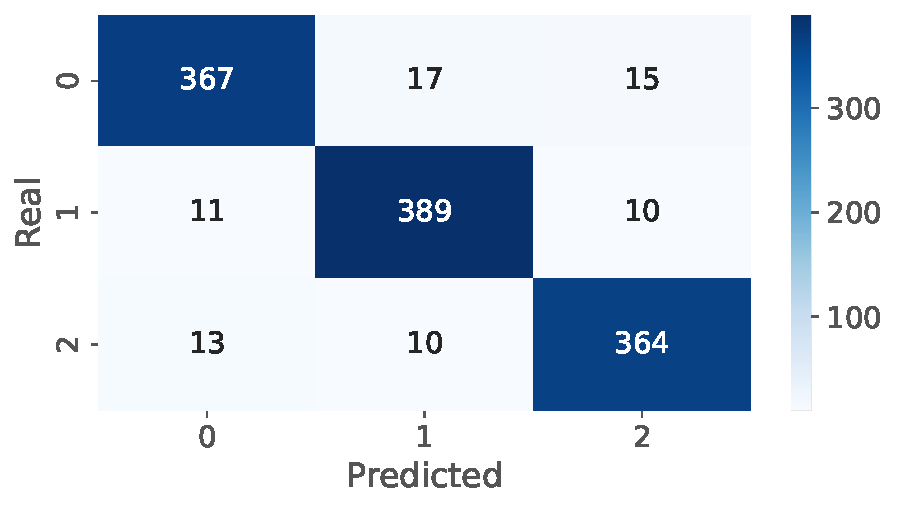
\includegraphics[width=.46\linewidth]{Figures/confusion_matrix_train.pdf}
            }
            \caption{Confusion matrices for the routing mechanism on the training and test datasets (0: first aid, 1: owner's manuals, 2: traffic regulations).}
        
            \label{fig:confusion_matrix}
\end{figure}

On the training set, the router reached an accuracy of 0.94. Precision, recall, and F1-score were 0.94 when averaged across classes, indicating that the Multinomial Naive Bayes model captures the lexical patterns associated with each domain.

On the test set, accuracy was 0.83, and macro-averaged precision, recall, and F1-score were also 0.83. The owner's manual class achieved a recall of 0.89, while first aid and traffic regulation reached 0.79 and 0.81, respectively. Most errors occur between first aid and traffic regulation, which suggests lexical overlap in the corresponding questions.

The gap between training and test performance is consistent with the dataset size and the BoW representation. The router maintains similar performance across classes without using neural gating. At the system level, routing errors affect only the queries for which the wrong expert is selected because the pipeline activates a single expert and does not aggregate outputs. These results indicate that a probabilistic router can support domain selection under MCU class compute and memory limits.


\subsection{SLM Expert and Global Model Evaluation}
\label{subsec:slm_expert_evaluation}

Figure~\ref{fig:radas_result} compares domain-specific experts (TinyMoE) with the Global Model. All metrics were normalized to the [0,1] range, where 1.0 represents the best result, such as lower cross-entropy or higher BLEU. For Cross-Entropy and Perplexity, inverse values were applied before normalization to ensure that higher scores indicate better performance.

\begin{figure}[htpb]
\centering
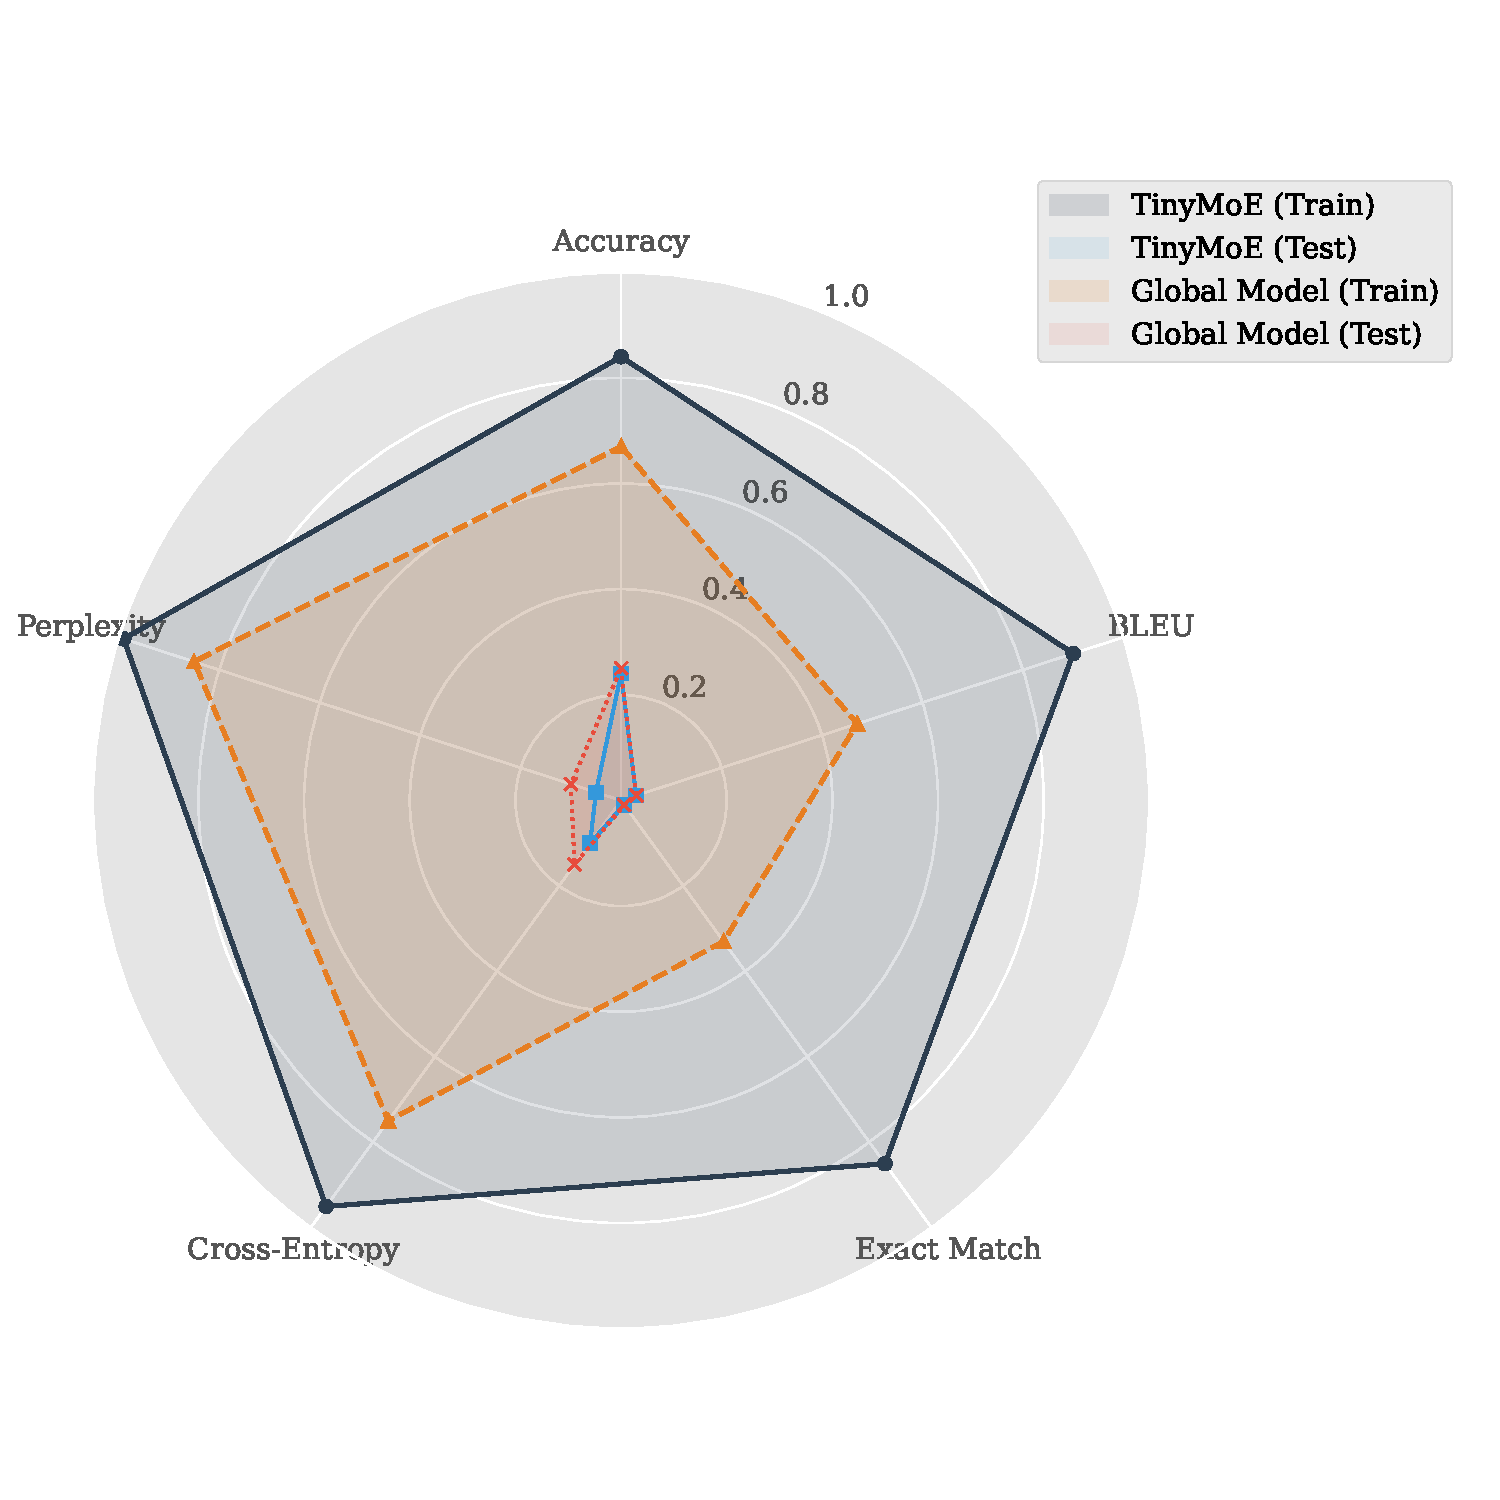
\includegraphics[width=.75\linewidth]{Figures/radar_complete_comparison2.pdf}
\caption{Performance profile of TinyMoE and the Global Model.}
\label{fig:radas_result}
\end{figure}

For the training split, represented by solid lines, TinyMoE outperforms the Global Model across all metrics, with larger gains in Exact Match and BLEU. This indicates that a single model has difficulty representing multiple domain-specific distributions. Higher normalized cross-entropy and perplexity scores also indicate lower training loss and uncertainty for TinyMoE.

For the test split, represented by dashed and dotted lines, both approaches show similar performance. TinyMoE maintains a slight advantage in token-level accuracy, while BLEU and Exact Match remain nearly identical. The Global Model achieves a slightly higher normalized cross-entropy score, suggesting a mild regularization effect from multi-domain training. This does not improve sequence-level performance and is associated with higher inference latency and lower memory locality.



\subsection{Edge Evaluation}
\label{subsec:edge_evaluation}

The deployment of TinyMoE across diverse MCUs reveals significant computational advantages over the monolithic Global Model. While the TinyMoE framework requires a larger Flash footprint to store specialized expert weights, its architectural efficiency translates into superior inference speeds across all tested platforms.

As shown in Fig.~\ref{fig:edge_result}, the TinyMoE approach consistently reduces inference latency. On the high-performance Arduino Portenta H7, TinyMoE achieves an inference time of 32.67~ms compared to 42.00~ms for the Global Model, representing a 22.2\% speedup. This trend is even more pronounced on mid-range hardware such as the ESP-32 and the Raspberry Pi Pico~2, where TinyMoE reduces latency by 36.7\% and 37.8\%, respectively. These gains are attributed to the routing mechanism, which allows the engine to process specialized sub-networks rather than accessing a saturated parameter space.

Memory management analysis indicates a strategic trade-off. TinyMoE exhibits a Flash memory overhead ranging from 21.5\% to 27.1\% due to the requirement of hosting multiple expert models. However, the RAM utilization during active inference remains optimized. For instance, on the Raspberry Pi Pico~2, TinyMoE demonstrates a high inference efficiency (134.33ms) despite the strict memory constraints of the ARM Cortex-M33 architecture. The most significant performance gap is observed in the standard Raspberry Pi Pico, where the Global Model's latency exceeds 3s, whereas TinyMoE remains 20.1\% faster, suggesting that specialized routing mitigates the computational bottlenecks inherent in M0\texttt{+} systems.

From a system-level perspective, these results validate that the MoE architecture is not only more accurate but also computationally more efficient. The marginal increase in storage (Flash) is a justifiable cost for the substantial reduction in inference latency, ensuring that SLMs can provide responsive assistance in critical embedded scenarios. 


\begin{figure}[htpb]
\centering
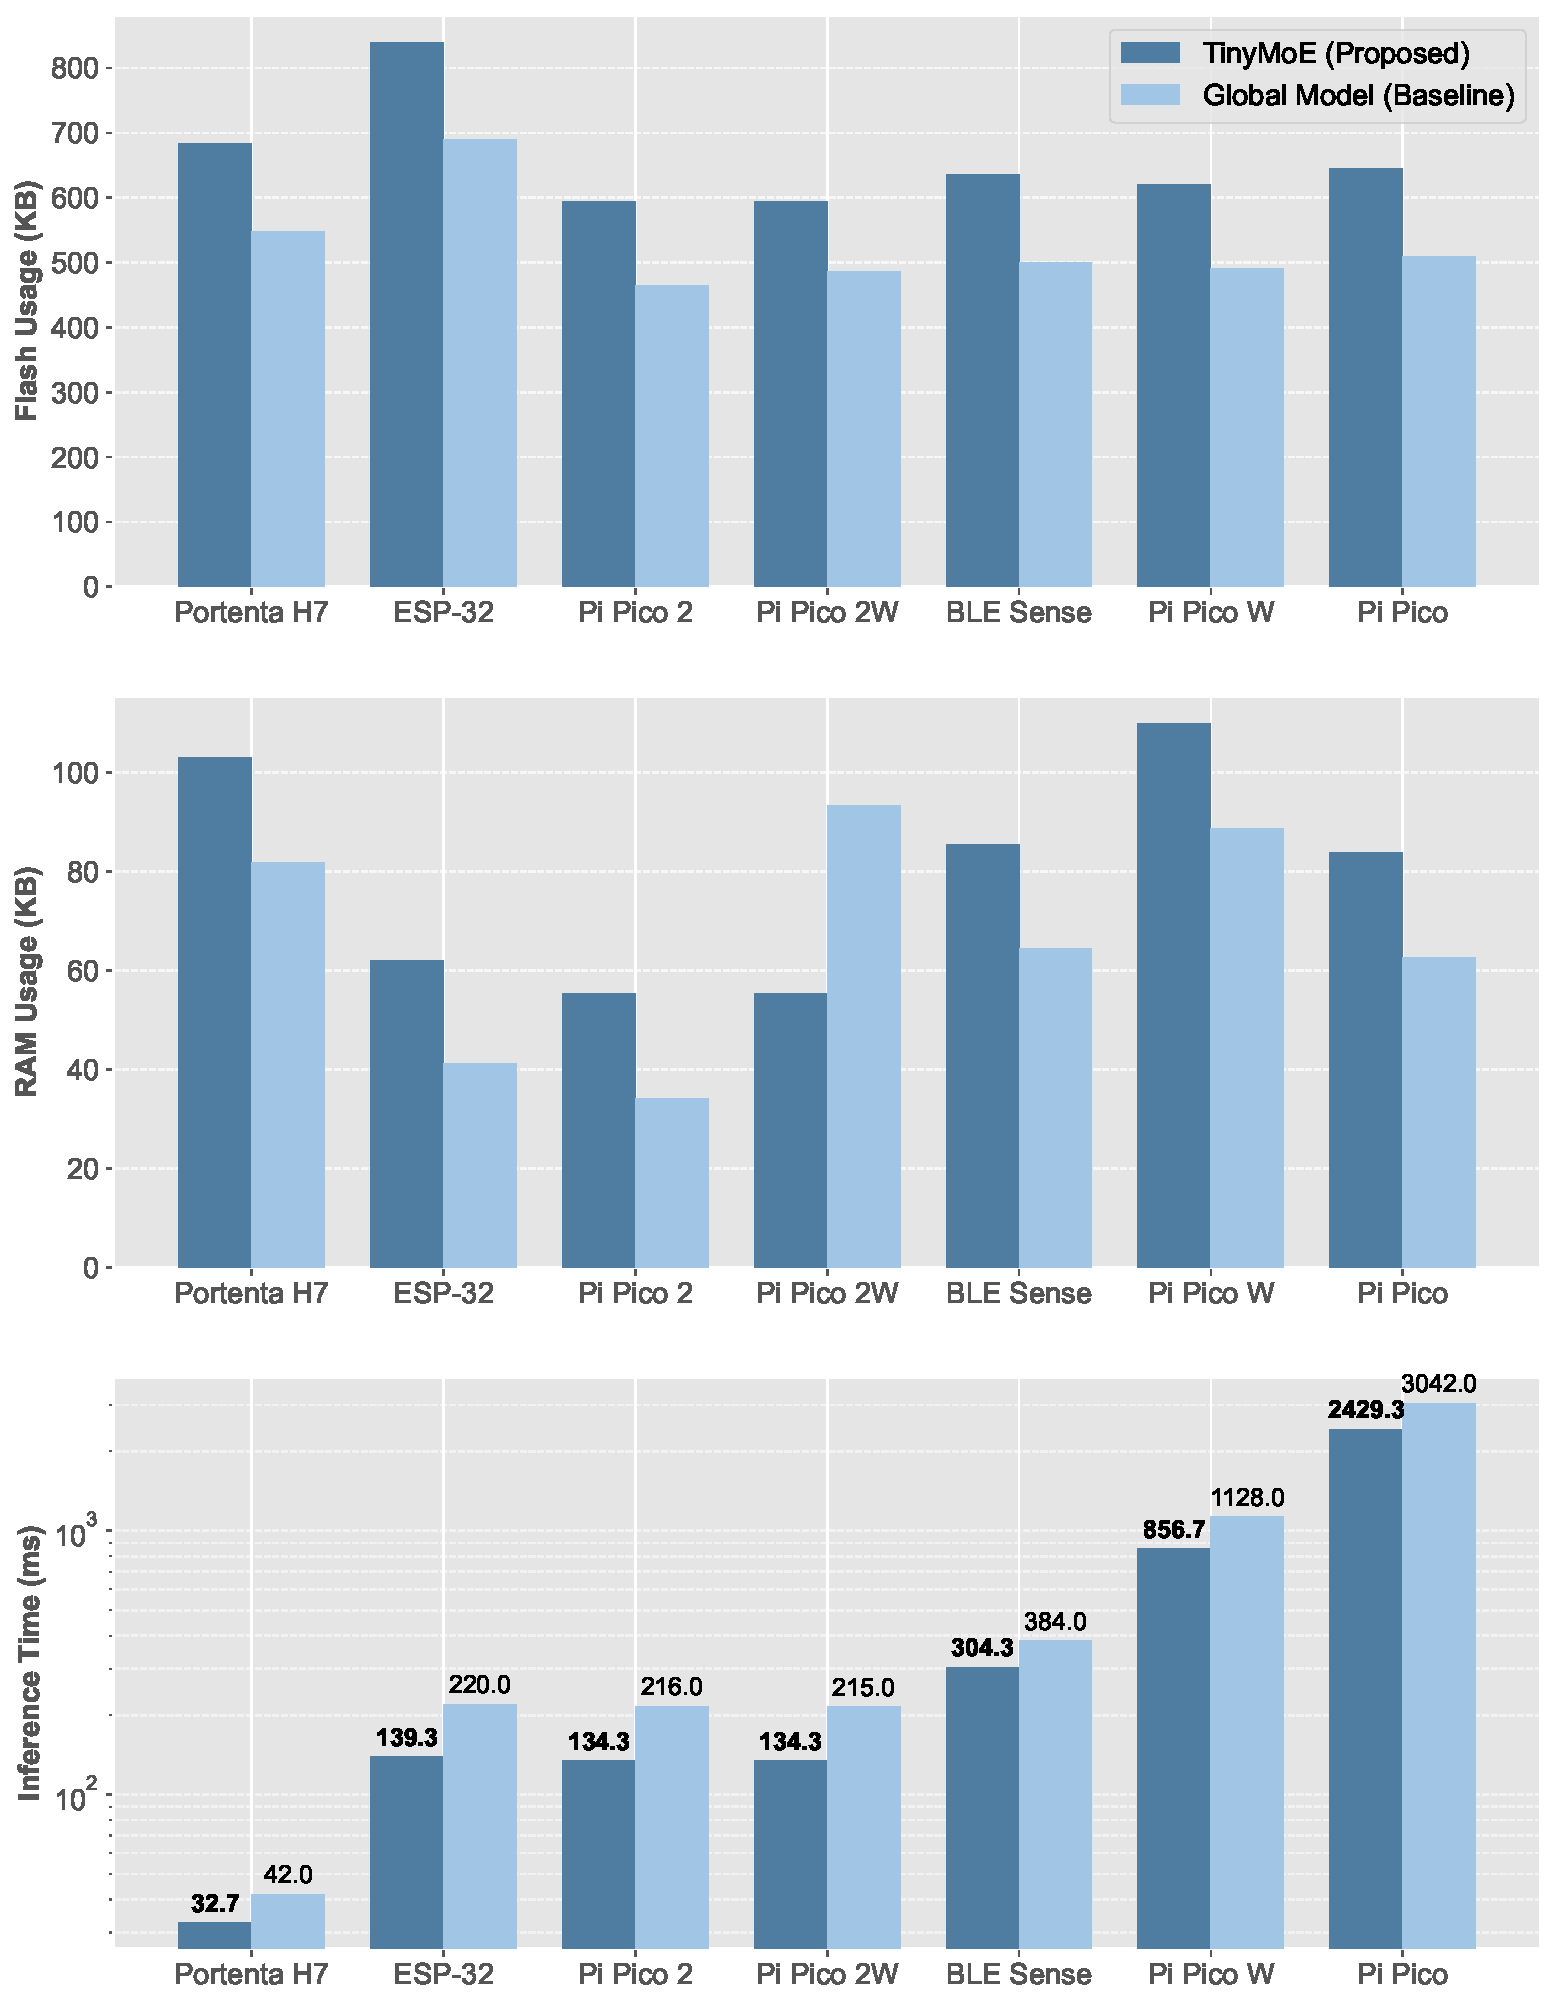
\includegraphics[width=.75\linewidth]{Figures/edge_performance_comparison.pdf}
\caption{Comparative performance analysis between TinyMoE and the monolithic Global Model across seven MCUs.}
\label{fig:edge_result}
\end{figure}


\section{Conclusion}
\label{sec:conclusion}

This paper presented TinyMoE, a modular Mixture-of-Experts architecture for natural language assistance in resource-constrained automotive systems. By enabling on-demand expert loading, TinyMoE can alleviate capacity saturation in monolithic SLMs. Experiments show that domain-specific experts significantly outperform a unified model, achieving a 116.3\% reduction in predictive uncertainty and nearly doubling alignment with training distributions.

Evaluations across multiple MCU platforms demonstrated that TinyMoE is both linguistically effective and computationally efficient. The semantic router provides over 30\% inference speedup on mid-range MCUs such as the ESP32 and Raspberry Pi Pico 2 while maintaining RAM usage suitable for bare-metal deployment. Although Flash storage overhead increases slightly, the resulting gains support real-time safety and diagnostic applications, with future work targeting adaptive quantization, scalable routing strategies, and the extension of the proposed architecture to handle multimodal.


\bibliographystyle{ieeetr}
\bibliography{References}

\end{document}
